\section{Chromatographic Feature Evaluation}\label{sec:feature_evaluation}
    For each candidate feature, we computed several metrics to estimate how distinguishable
    the observed signal was from random noise. We use the following quantities from each LC-MS
    feature:

    \renewcommand{\arraystretch}{1.5}
    \begin{table}
        \caption{Chromatogram Feature Definitions}\label{tbl:chromatogram_feature_definitions}
        \centering
        \begin{tabular}{l | p{9cm}}
            \hline
            $\mathcal{M}_i$          & The neutral mass of the $i$th chromatogram\\
            $\mathbfcal{I}_i$        & The total intensity array assigned to the $i$th chromatogram\\
            $\mathbfcal{I}_{i, j}$   & The sum of all peak intensities for peaks observed in
                                       the $j$th scan for the $i$th chromatogram\\
            $\mathcal{I}_{i, j, k}$  & The intensity assigned to the $k$th peak at the $j$th
                                       scan for the $i$th chromatogram\\
            $\mathbf{c}_i$           & The set of charge states observed for the $i$th chromatogram\\
            $\mathbfcal{I}_{i, c=j}$ & The total intensity assigned to the $i$th chromatogram
                                       with charge state $j$\\
            $\mathbf{t}_{i, j}$      & The time of the $j$th scan of the $i$th chromatogram\\
            $T_j$                    & The time of the $j$th scan of the experiment\\
            $\textbf{env}_{i, j, k}$ & The normalized experimental isotopic envelope composing
                                       the $k$th peak of the $j$th scan of the $i$th chromatogram,
                                       whose members sum to $1$\\
            $\mathbf{a}_i$           & The set of adduction states observed for the $i$th chromatogram\\
            $\mathbfcal{I}_{i, a=j}$ & The total intensity assigned to the $i$th
                                       chromatogram with adduct $j$\\
            ${\hat g}_i$             & The glycan composition assigned to the $i$th chromatogram, or \O
                                       \ if there was no matched glycan composition
        \end{tabular}
    \end{table}
    \renewcommand{\arraystretch}{1.0}

    All metrics are penalized by an $\epsilon = 1e-6$ to prevent scores from actually achieving
    a value of 1.0 which would make the logit value infinite. If a metric's value would be less
    than $0 + \epsilon$, it is given a value of $\epsilon$ instead to prevent the logit value from
    being undefined.

    \subsection{Chromatographic Peak Shape}
        An LC-MS elution profile should be composed of one or more peak-like components, each
        following a bi-Gaussian peak shape model (\cite{Yu2010}) or in less ideal chromatographic
        circumstances, a skewed Gaussian peak shape model. We fit these models using non-linear
        least squares (NLS). As measures of goodness of fit are not generally available for NLS,
        we use the following criterion:
        \begin{align}
            {\hat y_i} &= NLS(\mathbfcal{I}_i, \mathbf{t}_i) \nonumber\\
            e_{i, NLS} &= \mathbfcal{I}_i - {\hat y_i} \nonumber\\
            {\bar y_i} &= \mathbf{t}_i
                \left(
                    \left(
                        \mathbf{t}_i^t\mathbf{t}_i
                    \right)^{-1}\mathbf{t}_i\mathbfcal{I}_i
                \right)\nonumber\\
            e_{i, null} &= \mathbfcal{I}_i - {\bar y_i} \nonumber\\
            \mathscr{L}_i &= 1 - \frac{\sum{e_{i, NLS}^2}}{\sum{e_{i, null}^2}}
        \end{align}
        where line score describes how much the peak shape fit improves on a ordinary least squares
        regression linear model.

        We apply two competitive peak fitting strategies to address distorted, overlapping, or
        multimodal elution profiles. The first works iteratively by finding a best-matching peak
        shape using non-linear least squares, subtracting the fitted signal and checks if there is
        another peak with at least half as tall as the removed peak, if so repeating the process until
        no peak can be found, saving each peak model so constructed. The second approach starts
        by locating local minima between putative peaks, and partitioning the chromatogram into
        sub-groups which would are fit independently. This method generates a candidate list of
        minima, and selects the case which has the greatest difference between the minimum and its
        pair of maxima to split the feature at. The strategy which produces the maximum $\mathscr{L}_i$
        is chosen. $\mathscr{L}_i$ is bounded in $(-\infty, 1]$, where $1$ corresponds to a perfect
        fit, and 0 would correspond to the peak shape fit being no better than the OLS straight line
        fit. This metric is thresholded at 0.15, with any chromatogram scoring below 0.15 being
        discarded as having insufficient peak shape evidence to interpret.

    \subsection{Composition Dependent Charge State Distribution}
        % Does this principle need a citation?
        As the number of monosaccharides composing a glycan increases, the number of possible sites
        for charge localization increases. This relationship is visualized in Figure~\ref{fig:charge_trend_plot}.
        Under normal conditions, we would expect to observe the same molecule in multiple charge states
        (\cite{Maxwell2012}). Which charge states are expected would depend upon the size of the molecule
        and it's constituent units' electronegativity. In it's native state, \monosaccharide{NeuAc}'s
        acidic group causes glycans with one or more \monosaccharide{NeuAc} to have a propensity for
        higher negative charge states (\cite{Varki2009}). To capture this relationship, we modeled the
        probability of observing a glycan composition for sialylated and unsialylated compositions
        separately. For permethylated glycans, charge is carried by protons or metallic cation adducts
        like sodium, the relationship between acidic monosaccharides and charge state propensities is
        weaker.
        \begin{align}
            m_i &= (\floor*{(\mathcal{M}_i / w) / 10} + 1) * 10 \nonumber\\
            \mathcal{H}_{i,j} &= \frac{
                \mathbfcal{I}_{i, c=j}}{\mathbfcal{I}_i} \nonumber\\
            P(c, m) &= \frac{\sum_{m_i \in m} \mathcal{H}_{i, j}}{
                \sum_{j}{\sum_{m_i \in m} \mathcal{H}_{i, j}}} \nonumber\\
            \mathscr{C}_i &= \sum_{c_{i, j} \in \mathbf{c}_i}{P(c_{i, j}, m_i)}
        \end{align}
        where $w$ is the width of the mass bin divided by 10 and $P(c, m)$ is defined as
        part of the model estimation procedure. If the model is complete, then this metric is
        bounded within $[0, 1]$ where 0 corresponds to having no observed charge states and 1
        corresponds to all expected charge states being observed. In practice, the model is not
        complete, where an existing mass range may be missing a charge state in which case
        $P(c, m)$ is the average over all known values of $c$ in $m$. When a mass range is
        required but missing from the model, the model will fall back to a naive model where
        $P(c, m) = 0.4 \ \forall \ c$ and as such this metric must be clamped to not exceed
        1.0. This metric has an exceptional threshold of 0.05 instead of 0.15.

        \begin{figure}
            \centering
            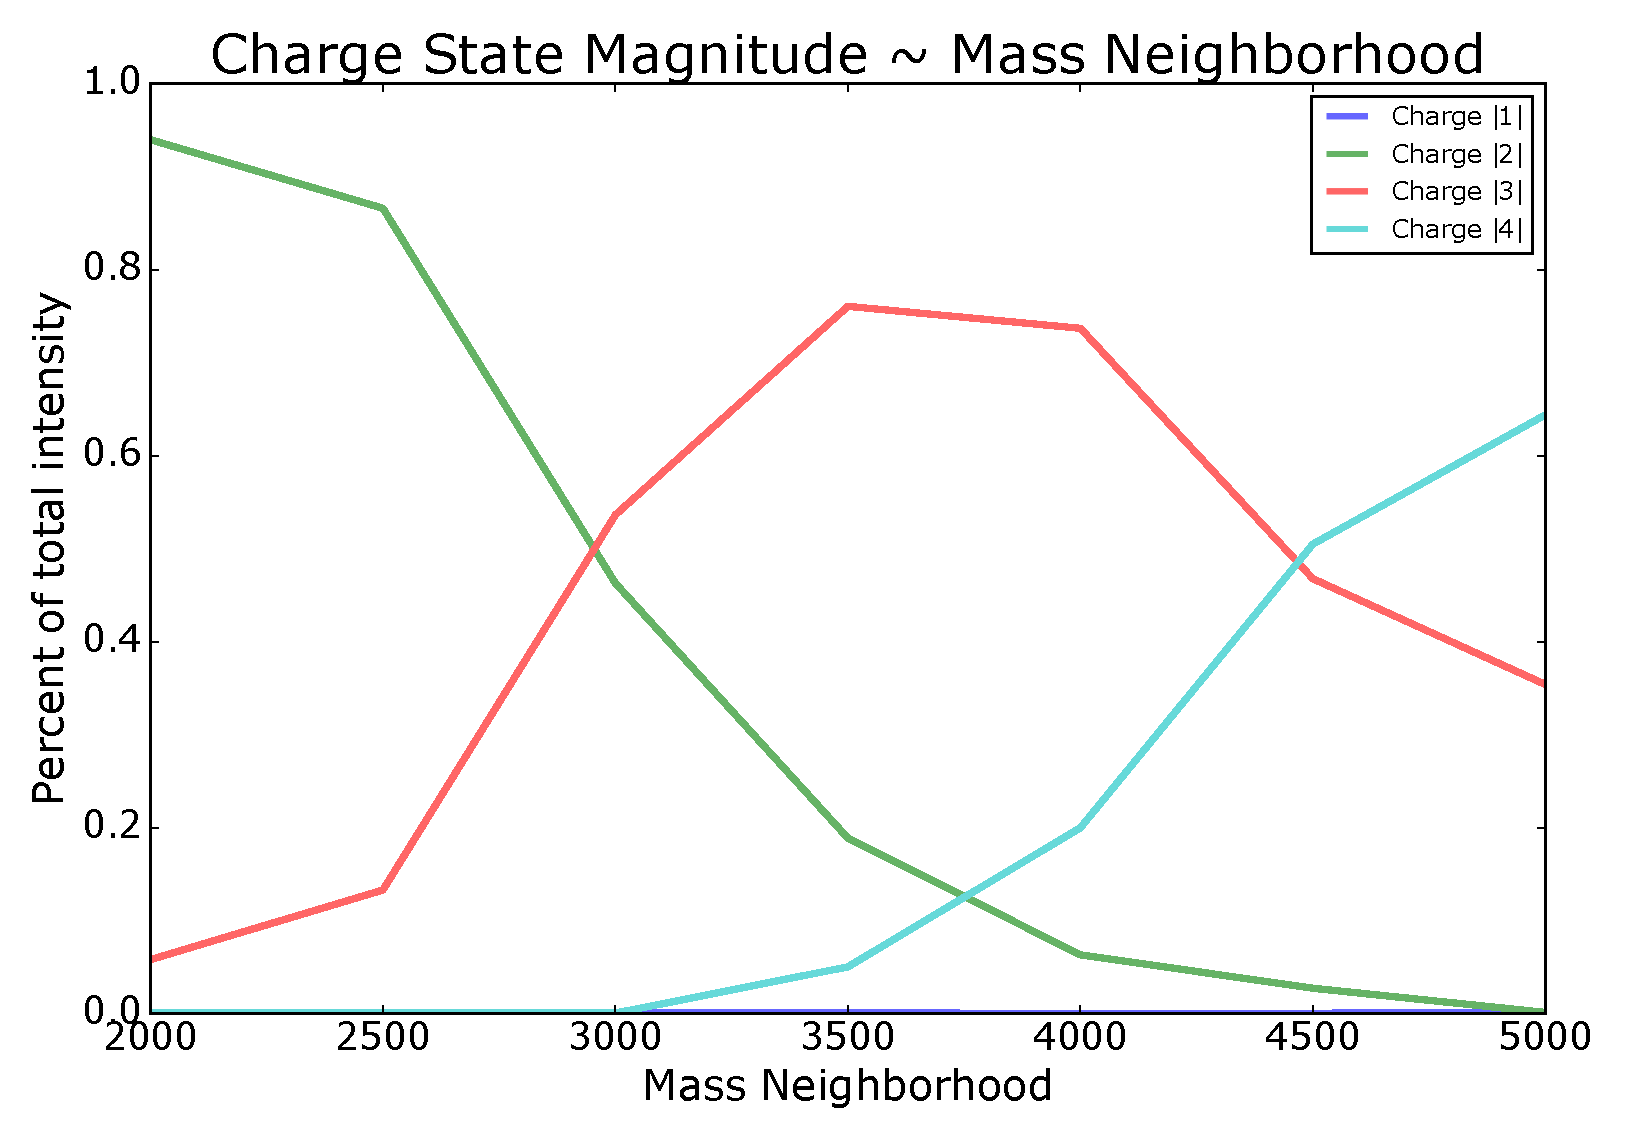
\includegraphics[width=0.75\linewidth]{figure/charge_trend_plot}
            \caption{The trend of charge state relative abundance for acidic glycans}
            \label{fig:charge_trend_plot}
        \end{figure}

    \subsection{Adduction Frequency}
        For the datasets \textit{AGP-permethylated-2ul-inj-55-SLens} and \textit{Perm-BS-070111-04-Human-Serum}
        we also include an adduction frequency model score $\mathscr{A}_i$, following the same
        pattern as the charge state distribution, with the same extension of justification
        from \cite{Maxwell2012}. We use one mass scaling model for all glycan compositions
        as ammonium adduction is not expected to be composition dependent.
        \begin{align}
            m_i &= (\floor*{(\mathcal{M}_i / w) / 10} + 1) * 10 \nonumber\\
            \mathcal{H}_{i,j} &= \frac{
                \mathbfcal{I}_{i, a=j}}{\mathbfcal{I}_i} \nonumber\\
            P(a, m) &= \frac{\sum_{m_i \in m} \mathcal{H}_{i, j}}{\sum_j{
                \sum_{m_i \in m} \mathcal{H}_{i, j}}} \nonumber\\
            \mathscr{A}_i &= \sum_{a_{i, j} \in \mathbf{a}_i}{P(a_{i, j}, m_i)}
        \end{align}
        We fit an ammonium adduction model on \textit{AGP-permethylated-2ul-inj-55-SLens}
        in order to make our comparison to third-party data less biased given limited sample data.
        This metric is bounded within $[0, 1]$ where 0 corresponds to having no observed adduction
        states within the model and 1 corresponds to all observing all adduction states in the model.
        This metric follows the same behavior as the charge state distribution metric w.r.t. missing
        information within the model, but will reject chromatograms when this metric score is below 0.15.

        We fit a sialylation-aware formate adduction model on a collection of sialylated and unsialylated
        native \nglycan samples from replicates of the \agp, \igg, and \phil datasets. This model was used
        for \agp, \igg, \phil and \philbs. This model had its upper limit set to 0.7, so it could not contribute
        a large positive number to the score of a match after logit transformation. This is desirable because
        we want to be able to eliminate matches which are made with improbable formate adducts when no
        reasonable adduction state is present.

    \subsection{Isotopic Pattern Consistency}
        Our ahead-of-time deconvolution procedure uses an averagine isotopic model and does not
        capture the consistency of the isotopic pattern that was fit with the isotopic pattern
        of the glycan composition that matched that peak. The criterion
        \begin{align}
            \mathscr{I}_i &= 1 - 2\mathbfcal{I}_i^{-t}\mathbf{I}_i\sum_j^J{
                \sum_k^K{\mathcal{I}_{i, j, k}
                    \textbf{env}_{i, j, k}^t\left(
                        \ln{\textbf{env}}_{i, j, k} -
                        \ln{\textbf{tid}_{i}}
                    \right)
                }
            }
        \end{align}
        where \textbf{tid} is the theoretical isotopic pattern derived from either ${\hat g}_i$
        or an averagine interpolated for $\mathcal{M}_i$ if ${\hat g}_i =$ \O and any mass shifting molecular
        adduct or neutral loss for the matched peak. This computes a per-peak intensity weighted mean
        G-test comparing the goodness of fit between the experimental envelope and the theoretical
        isotopic pattern. This metric is bounded within $(-\infty, \infty)$ as the G-test achieves
        its optimal value at 0, and can take on extreme values towards either signed $\infty$, however
        because of the previous deconvolution process, in practice it cannot take on such extreme
        values and is bounded within $(-\infty, 1]$. This metric is thresholded at 0.15, with any
        chromatogram scoring below 0.15 being discarded as having insufficient isotopic consistency
        to interpret.

    \subsection{Observation Spacing Score}
        The less time between observations of a glycan composition the less likely the chromatogram
        is to contain peaks missing or caused by isotopic pattern interference or missing information.
        \begin{align}
            d_i &= \frac{1}{T_i - T_j} \nonumber\\
            \mathscr{T}_i &= 1 - 2\mathbfcal{I}_i^{-t}\mathbf{I}_i\sum_{j=1}^J\mathbfcal{I}_{i, j}
                             f\left(d_i\left(\mathbf{t}_{i, j} - \mathbf{t}_{i, j - 1}\right)\right)
        \end{align}
        As this metric depends heavily on the speed of the mass spectrometer, a scaling function $f$
        must be estimated from the total ion chromatogram to reduce the penalty on slower instruments.
        When $\frac{1}{J}\sum_{j}^{J}{T_j - T_{j - 1}} > 0.2$, $f(x) = x / \left(\frac{1}{J}
        \sum_{j}^{J}{T_j - T_{j - 1}} * 15\right)$, otherwise $f(x) = x$. This metric is bounded within
        $(-\infty, 1]$ as $\left(\mathbf{t}_{i, j} - \mathbf{t}_{i, j - 1}\right)$ is always positive.
        This metric is thresholded at 0.15, with any chromatogram scoring below 0.15 being discarded
        as having insufficient detection consistency to interpret.

    \subsection{Summarization Score}
        Each scoring metric $\in \left[\mathscr{L}_i, \mathscr{C}_i, \mathscr{I}_i,
        \mathscr{T}_i, \mathscr{A}_i\right]$ is penalized by $\epsilon = 1\mathrm{e}{-6}$ bounded in
        the range $[0, 1)$, with values below 0 set to $\epsilon$.
        \begin{align}
            s_i &= \sum_{f_{i,j} \in \text{features}_i}{\ln{
                \frac{f_{i, j}}{1 - f_{i, j}}
                }
            }
        \end{align}
        producing a value between $(-\infty, \infty)$. $s_i < 8$ reflects multiple
        poor scores and is unexpected to be real, while $s_i > 15$ is
        consistent with model expectations.

\begin{table}
        \caption{Score Thresholds}\label{tbl:feature_score_thresholds}
        \centering
        \begin{tabular}{l | S}
            \hline
            Chromatographic Peak Shape & 0.15 \\
            Charge State Distribution & 0.05 \\
            Adduction Frequency & 0.15 \\
            Isotopic Pattern Consistency & 0.15 \\
            Observation Spacing & 0.15 \\
        \end{tabular}
    \end{table}